\chapter{Расчетные исследования известных схем}\label{ch:ch2}

Начнем с очерчивания рамок расчетного исследования.
Оставляя в стороне вопросы, связанные с химической переработкой для получения восстановленной урановой изотопной смеси, предлагается рассмотрение усовершенствованных каскадов газовых центрифуг для повторного обогащения этой смеси для производства низкообогащенного урана. 

В расчетных задачах ограничимся следующими предположениями:

 \begin{enumerate}
  \item регенерированный ураном, получен из ОЯТ легководного энергетического реактора. В качестве примера будем рассматривать изотопный состав регенерата из реактора российского дизайна -- ВВЭР.
  \item коэффициент разделения характерен центрифуге российского дизайна.
\end{enumerate}

\section{Обоснование ограничений использования ординарных схем (на основе ординарных каскадов)}\label{sec:ch2/sec1}


Таким образом, анализ схем на основе базового трехпоточного каскада демонстрирует потребность в модификации компоновок разделительного оборудования в контексте многократного рецикла урана.

Подводя итог подраздела, известные на сегодняшний день  технические решения основаны на:
-	разбавлении регенерированного урана материалами, не содержащими минорных компонентов (например, природным ураном), на входе в разделительный каскад, на выходе из разделительного каскада или внутри каскада при наличии в нем двух питающих потоков (регенерат и разбавитель);
-	получении регенерата с пониженным содержанием минорных изотопов в каскаде с двумя питаниями и двумя потоками продукта (отбора);
-	выделении из смесей регенерированного урана изотопа $^{232}$U при помощи газа-носителя в последовательном соединении двух разделительных каскадов.

\section{Обоснование необходимости составных схем/схем с дополнительными потоками}\label{sec:ch2/sec2}
Из вышепреведенного обоснования невозможности решения задачи полного возврата регенерата в топливный цикл легководных реакторов в условиях многократного рецикла и вытекает необходимость использовать составные каскадные схемы ввиду необходимости  <<пространственного>> разделения. Так двойная схема позволяет отделить минорные легкие изотопы $^{232}$U, $^{234}$U в независимом потоке отборной части каскада.
Так, например, схема \ref{fig:double} позволяет во втором каскаде разделить потоки, выделив $^{235}$U в тяжелой фракции, направив $^{232}$U и $^{234}$U в легкую.

\begin{figure}[ht]
  \centerfloat{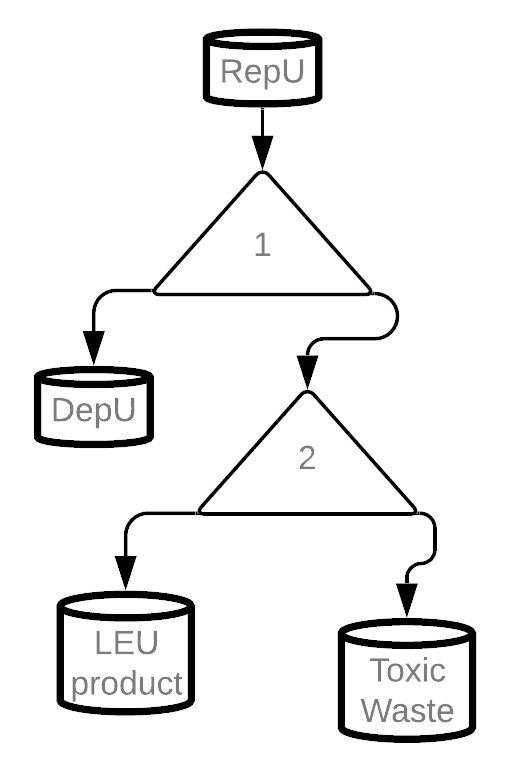
\includegraphics[scale=0.3]{cascades/double}}
  \caption{Двойной каскад}\label{fig:double}
\end{figure}

С появлением свойств такого рода у каскадов, вместо привычной дихотомии, выделяющей схемы с приставкой <<много->> (многопоточные схемы, многокаскадные конфигурации), предлагается классифицировать каскады, используемые для обогащения регенерата, как разбавляющие или очищающие. Так, схема двойного каскада является очищающей, в отличие от схем, основанных на ординарном каскаде, работающих на принципе разбавления.  Хоть и любая таксономия арбитрарна
% (\textcolor{red}{позиция номиналистов в споре с реалистами})
, условная граница `каскад-разбавитель' -- `каскад-очиститель' гораздо лучше подчеркивает сущностные характеристики анализируемых схем, предназначенных для повторного обогащения урана.
 

\section{Разработка схем полного возврата}\label{sec:ch2/sec3}
\subsection{Модифицированный двойной каскад}

В качестве модификации двойного каскада была предложена альтернативная каскадная схема, которая позволяет обеспечить возврат регенерата в цикл в соотношении 1:1. В этой схеме, изображенной 
на рисунке \ref{fig:vestnik}, первая часть (каскад 1) увеличивает 
концентрацию $^{235}$U со всеми более легкими изотопами ($^{232}$U и $^{234}$U) и направляет их (через выходящий поток в правой части на рисунке) ко второму каскаду, который будет концентрировать эти четные миноры в потоке загрязненного продукта \cite{smirnovObogashchenieRegenerirovannogoUrana2018}.
Хотя на этот раз приготовленная композиция разбавляется НОУ для контроля концентраций $^{232}$U и $^{234}$U в допустимых пределах и для управления соотношением рециклируемых материалов (для поддержания соотношения регенерата в питании каскада к нарабатываемому продукту на уровне 1:1, что формально соответствует полному возврату выгоревшего топлива в ядерный топливный цикл).

\begin{figure}[ht]
  \centerfloat{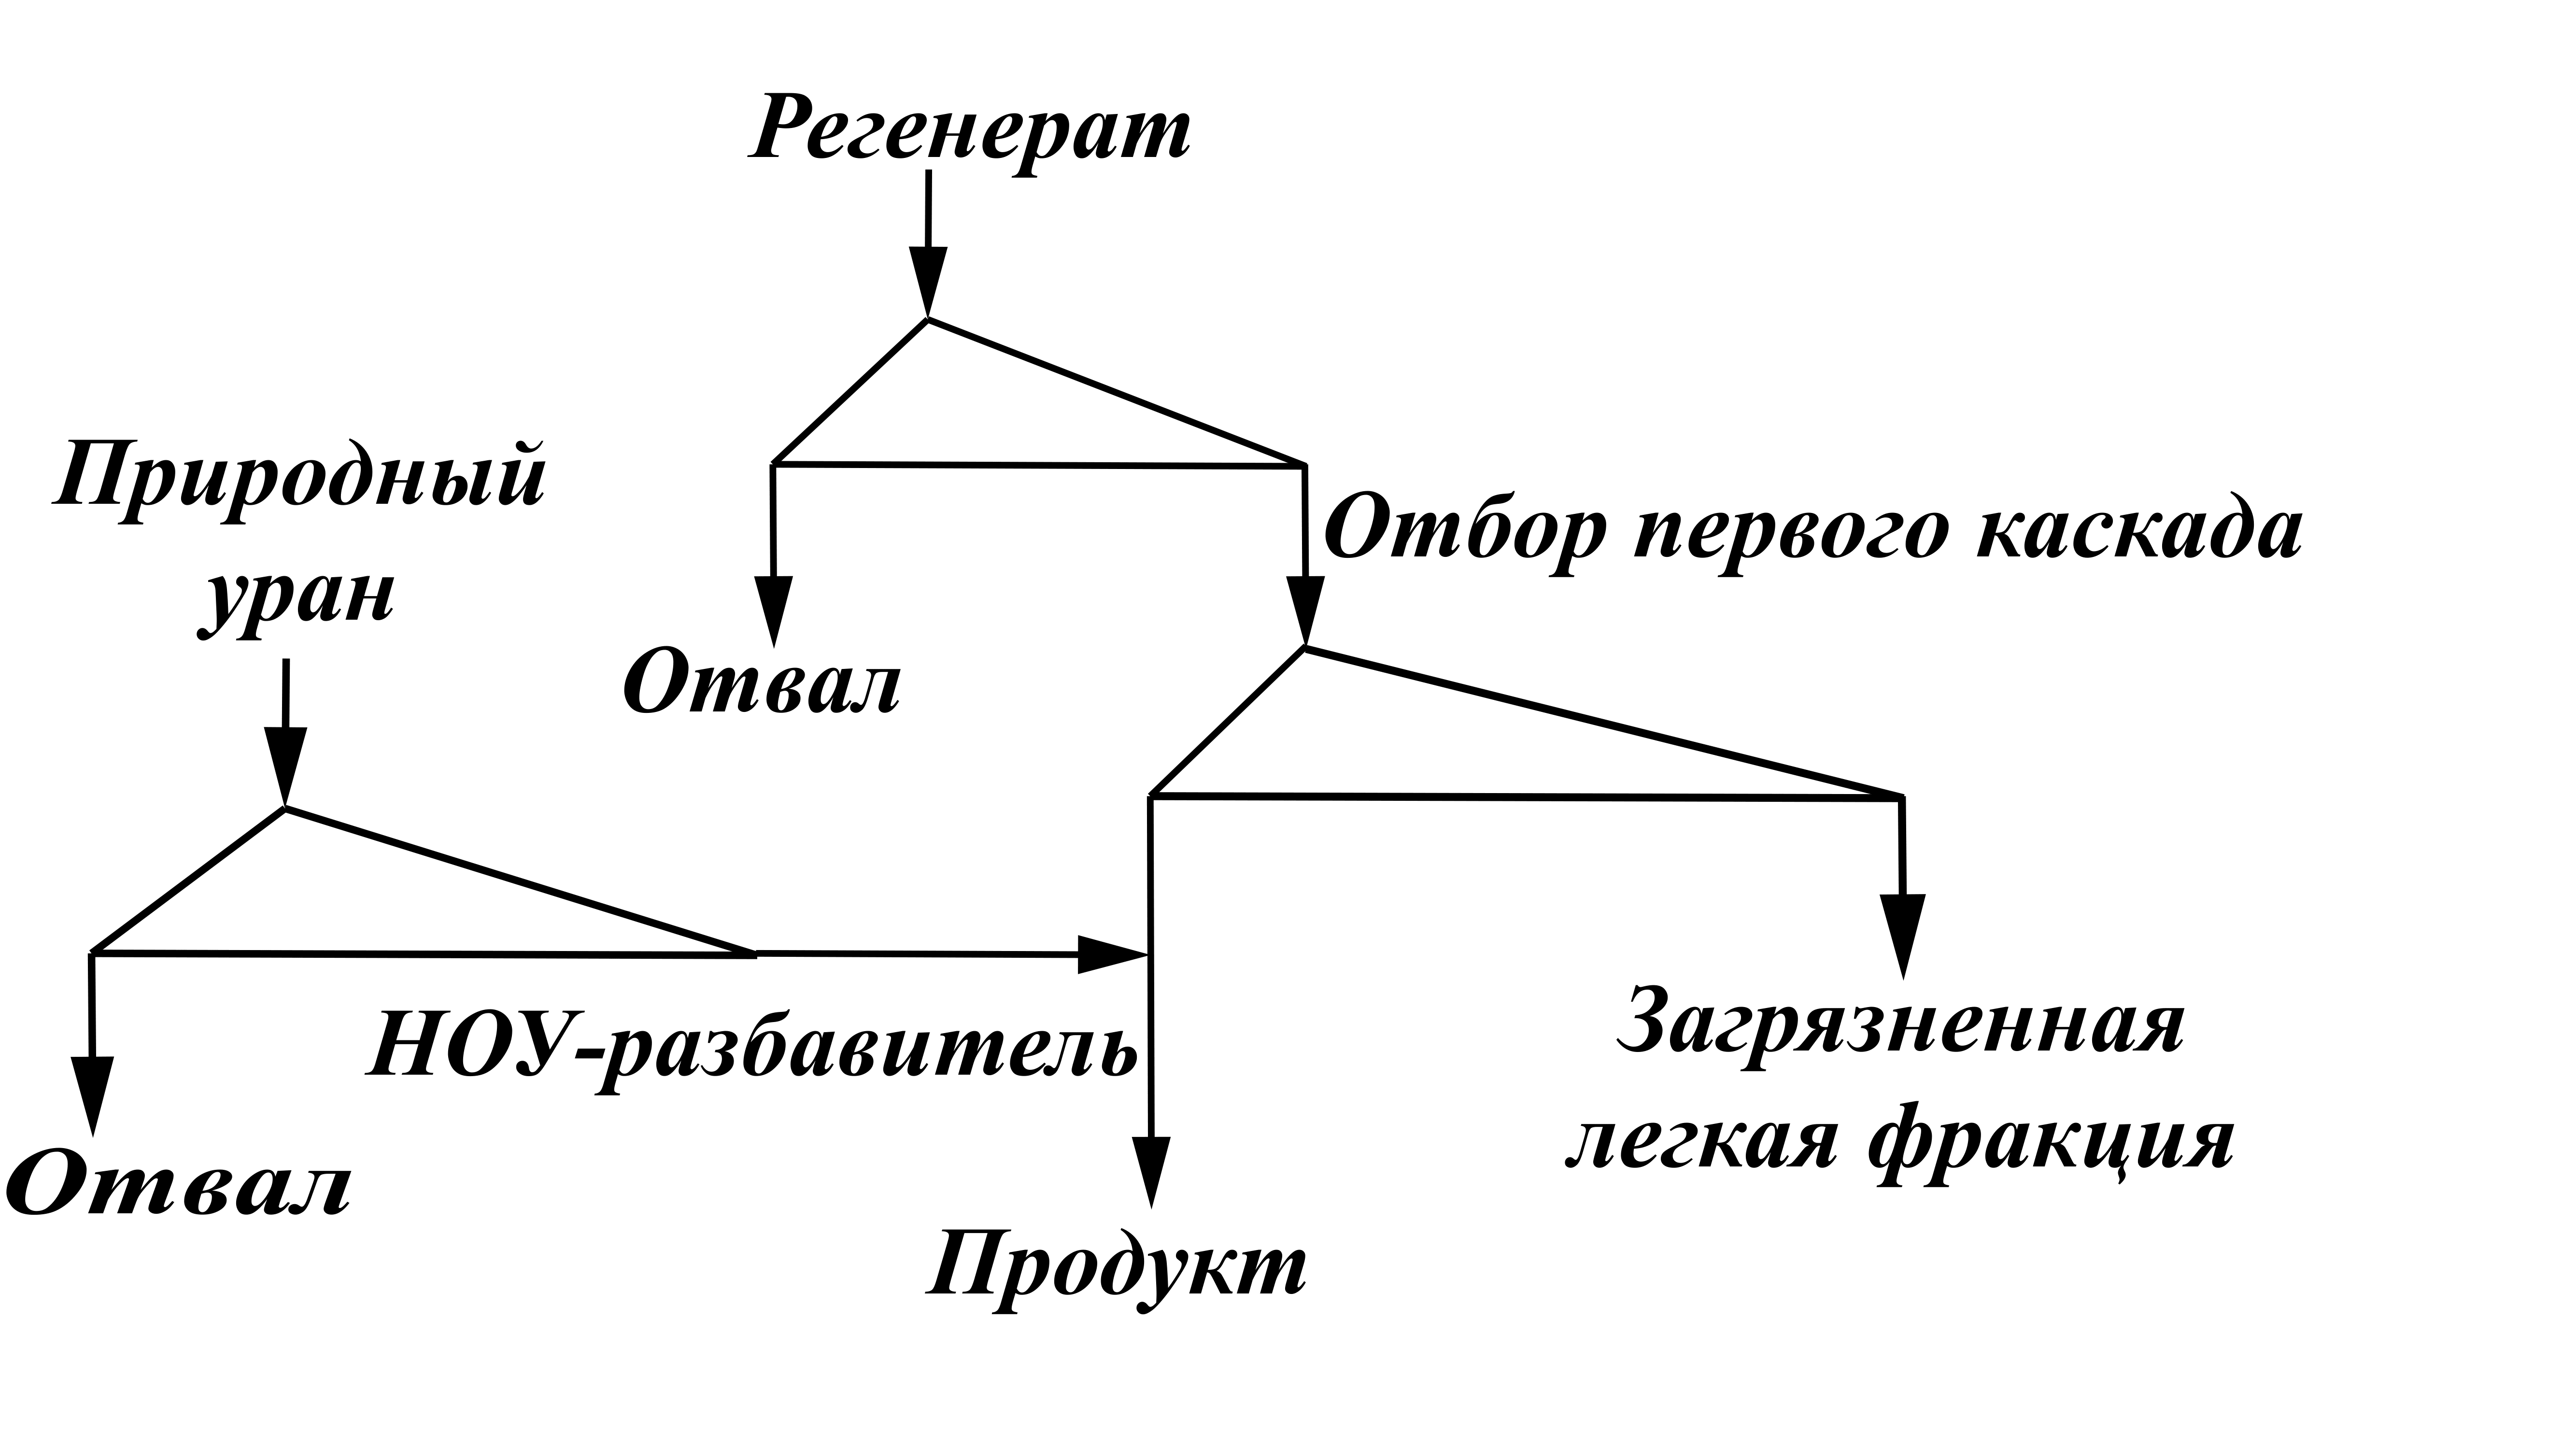
\includegraphics[scale=0.1]{cascades/triple}}
  \caption{Двойной каскад с добавлением НОУ (тройной каскад)}\label{fig:vestnik}
\end{figure}

Отличие предлагаемой схемы от двойного каскада состоит в том, что поток отвала второго каскада не является конечным продуктом.
Финальным шагом получения товарного продукта является разбавление этого потока сырьём, не содержащим искусственных изотопов урана с целью их разбавления и, соответственно, обеспечения заданных ограничений по $^{232,236}$U.
Для выполнения условия полного возврата регенерата в цикл отношение потоков НОУ-разбавителя и отвала второго каскада, которые образуют товарный продукт, является предопределённым, поскольку при заданной концентрации выходящих потоков обоих каскадов известным является отношение потока тяжелой фракции второго каскада к питающему регенерату, и при этом условиями задачи предопределено отношение потока исходного регенерата к конечному-НОУ.
В этом случае единственным параметром, позволяющим влиять на концентрацию $^{235}$U в товарном продукте, является концентрация данного изотопа в разбавителе (в потоке НОУ-разбавитель на рис. \ref{fig:vestnik}).
Таким образом, величину обогащения $^{235}$U в потоке этого разбавителя подбирают для конкретных заданных внешних условий \cite{smirnovObogashchenieRegenerirovannogoUrana2018}.

Очевидно, что поскольку питанием первого каскада является исходный регенерат, питанием второго -- полученный из него среднеобогащённый регенерат, то поток тяжёлой фракции на выходе из второго каскада будет по величине в несколько раз меньше, чем исходный поток регенерата. Такая работа каскада обеспечивает перерасход регенерата на единицу продукта. Следовательно, поток разбавителя должен в несколько раз превосходить по величине поток тяжелой фракции второго каскада. Однако, если в качестве разбавителя использовать, например, природный уран, это условие может привести к снижению концентрации $^{235}$U ниже требуемой величины. Если же в качестве разбавителя использовать низкообогащённый уран, то можно увеличить отношение потоков НОУ-разбавителя к <<отвалу>> второго каскада, доведя ее до требуемого значения.  
Такая схема близка к описанной в патенте \cite{zhurinSposobIzotopnogoVosstanovleniya2010}. Однако отличием предлагаемого двойного каскада является то, что ни в одном из каскадов в схеме не происходит превышение концентра-ции $^{235}$U выше значения 20\%. При этом в схеме  \cite{zhurinSposobIzotopnogoVosstanovleniya2010} концентрация $^{235}$U в потоке P1 достигает 90\% и более. Кроме того, величина отношения потока регенерата к конечному продукту на рис. \ref{fig:vestnik} всегда является строго заданной, что позволяет расходовать на получение заданного количества продукта требуемое количество регенерированного урана.

Итак, согласно \cite{smirnovObogashchenieRegenerirovannogoUrana2018} схема, представленная на рис. \ref{fig:vestnik}, позволяет обогатить регенерированный уран, полученный после пяти рециклов в топливе реакторов ВВЭР-1000 при соотношении расхода регенерата и продукта 0,93 и ограничении на концентрацию $^{232}$U $5\cdot10^{-7}$\%. Представляет интерес анализ возможности обогащения регенерата в такой схеме при заданном соотношении между массами исходного регенерата и продукта больше единицы. Такое заданное условие моделирует ситуацию обогащения и вовлечения в воспроизводство топлива регенерированного урана, накопленного к текущему моменту за период эксплуатации легководных реакторов. Дополнительный интерес представляет анализ поведения характеристик по-добной схемы в зависимости от ограничений на концентрацию изотопа $^{232}$U в продукте. 

\subsubsection{Анализ влияния ограничений предельно допустимой концентрации $^{232}$U в товарном НОУ}

Далее представлены результаты расчёта параметров модификации двойного каскада, представленной на рис. \ref{fig:vestnik}, для различных ограничений на концентрацию изотопа $^{232}$U в продукте, а также соотношения между расходами исходного регенерата и получаемым товарным НОУ.
Согласно цели диссертации, состоящей в исследовании возможностей полного возврата регенерата в режиме многократного рецикла, в качестве сырья для обогащения был рассмотрен регенерированный уран, испытавший несколько циклов облучения (табл. \ref{RepU_fifth}) \cite{palkinDesignanalyticalResearchRefinement2010}.

\begin{table}
  \begin{tabular}{c|c|c} 
  \hline
  Номер компонента & Массовое число & Концентрация, $\%$ \\
  \hline 1 & 232 & $1,03 \cdot 10^{-6}$ \\
  2 & 233 & $1,30 \cdot 10^{-6}$ \\
  3 & 234 & $3,91 \cdot 10^{-2}$ \\
  4 & 235 & 1,07 \\
  5 & 236 & 1,45 \\
  6 & 238 & Остальное \\
  \hline
  \end{tabular}
\caption{Состав обогащаемого регенерированного урана}\label{RepU_fifth}
\end{table}

Расчёты проведены при следующих условиях: обогащение по изотопу $^{235}$ составляло 4,95\%; относительный коэффициент разделения компонентов $^{235}UF_6$ и $^{238}UF_6$ принят равным 1,2 \cite{smirnovObogashchenieRegenerirovannogoUrana2018}; предельно допустимая концентрация изотопа $^{232}$ в НОУ не должна превышать величины $5\cdot10^{-7}$\%, $2\cdot10^{-7}$\%,$1\cdot10^{-7}$\%; потеря реактивности из-за присутствия $^{236}$ скомпенсирована добавочным обогащением по $^{235}$. Заданный расход регенерированного урана на единицу продукта принят равным:
а) 0,93 кг на 1 кг,
б) 1,86 кг на 1 кг продукта.
Цели расчетов:
\begin{enumerate}
  \item оценка возможности применения рассматриваемой схемы для указанных условий;
  \item оценка влияния изменения внешних условий на интегральные параметры рассматриваемого двойного каскада.
\end{enumerate}

В качестве расчётной модели в настоящей работе использована модель <<квазиидеального>> каскада \cite{sazykinKvaziidealnyeKaskadyDlya2000} с несмешиванием по относительным концентрациям выбранной пары компонентов (R-каскада) \cite{sulaberidzeTeoriyaKaskadovDlya2011}.
Ключевые интегральные характеристики для сравнения: удельный расход природного урана, удельные затраты работы разделения и отношение потоков P2/P0. В приведённых ниже результатах под работой разделения имели в виду условную величину, пропорциональную числу газовых центрифуг в каскаде. 

% Концентрацию 235U в потоке P1 варьирова-ли в пределах 5—20% с шагом 1%, в качестве рабочего значения для каждого случая выбира-ли величину, обеспечивающую выполнение ограничения на содержание 235U в разбавителе, полученном из природного урана, не более 5,0%. Для такого значения будет наблюдаться минимум по затратам работы разделения, эко-номии природного урана и отношению потоков P2/P0. Последнее условие означает, что будет произведено наименьшее количество загряз-нённого 232,234U изотопами материала P2, хране-ние которого требует определённых процедур, поскольку он представляет собой повышенную по отношению к штатным отходам раздели-тельных производств опасность.
При этом в каждом каскаде были выбраны следующие пары компонентов, по которым было выполнено условие несмешивания их относительных концентраций: первый каскад $^{235}$/$^{236}$, второй каскад $^{235}$/$^{234}$.

В табл. \ref{table_PDK_double_modified} представлены результаты расчёта изотопных составов,
в табл. \ref{table3_PDK_double_modified} -- удельный расход природного урана и интегральные характеристики экономии природного урана и перерасхода работы разделения по сравнению с ординарным каскадом, питаемым природным ураном, получающим продукт с эквивалентной эффективной концентрацией $^{235}$U (табл. \ref{table3_PDK_double_modified}). Под работой разделения понимается условная величина, пропорциональная числу газовых центрифуг в каскаде.
 Далее представлены соотношения получаемого загрязненного потока легкой фракции второго каскада к итоговому продукту.

\begin{table}
\begin{tabular}{|c|c|c|c|}
  \hline \multirow{2}{*} {Maccoвoe число} & 
  \multicolumn{3}{|c|}
  {Ограничение по изотопу $^{232} \mathrm{U}$, $\times 10^{-7}$} \\
  \cline {2-4} & 1 & 2 & 5 \\
  \hline \multicolumn{4}{|c|} { Случай $1\left(E_{1} / P_{0}=0,93\right)$} \\
  232 & $1,00 \cdot 10^{-7}$ & $2,00 \cdot 10^{-7}$ & $5,00 \cdot 10^{-7}$ \\
  233 & $2,12 \cdot 10^{-7}$ & $3,62 \cdot 10^{-7}$ & $7,41 \cdot 10^{-7}$ \\
  234 & $4,90 \cdot 10^{-2}$ & $5,30 \cdot 10^{-2}$ & $6,21 \cdot 10^{-2}$ \\
  235 & 5,06 & 5,09 & 5,14 \\
  236 & $3,70 \cdot 10^{-1}$ & $4,67 \cdot 10^{-1}$ & $6,61 \cdot 10^{-1}$ \\
  \multicolumn{4}{|c|} { Случай $2\left(E_{1} / P_{0}=1,86\right)$} \\
  232 & $1,00 \cdot 10^{-7}$ & $2,00 \cdot 10^{-7}$ & $5,00 \cdot 10^{-7}$ \\
  233 & $2,40 \cdot 10^{-7}$ & $4,12 \cdot 10^{-7}$ & $8,55 \cdot 10^{-7}$ \\
  234 & $5,09 \cdot 10^{-2}$ & $5,60 \cdot 10^{-2}$ & $6,79 \cdot 10^{-2}$ \\
  235 & 5,10 & 5,15 & 5,24 \\
  236 & $5,26 \cdot 10^{-1}$ & $6,73 \cdot 10^{-1}$ & $9,85 \cdot 10^{-1}$ \\
  \hline
  \end{tabular}
  \caption{Изотопные составы продукта в модифицированном двойном каскаде для различных условий}\label{table_PDK_double_modified}
\end{table}

\begin{table}
\begin{tabular}{|c|c|c|c|c|}
  \hline
  \makecell{$^{235}$U в \\ потоке  \\ отбора  \\первого  \\каскада, \%} & \makecell{Экономия \\природного  \\ урана, \%} & \makecell{Перерасход \\ работы  \\ разделения, \%} & \makecell{Отношение \\ потока  отбора \\второго каскада \\ к продукту}
  & \makecell{Ограничение  \\ по изотопу $^{232}$U \\ , $\times 10^{-7}$} \\
  \hline
  \multicolumn{5}{|c|} {Случай $1\left(E_{1} / P_{0}=0,93\right)$} \\
  11 & 4,9 & 17,2 & 0,02785 & 1 \\
  10 & 6,7 & 14,7 & 0,02201 & 2 \\
  8 & 10,3 & 9,7 & 0,01038 & 5 \\
  \multicolumn{5}{|c|} { Случай $1\left(E_{1} / P_{0}=0,93\right)$} \\
  13 & 6,6818 & 39,0985 & 0,06648 & 1 \\
  12 & 9,2857 & 35,4797 & 0,05798 & 2 \\
  10 & 14,7795 & 27,7759 & 0,04005 & 5 \\
  \hline
  \end{tabular}
  \caption{Интегральные параметры рассматриваемого двойного каскада для различных внешних условий}\label{table3_PDK_double_modified}
\end{table}


Анализ результатов таблицы \ref{table_PDK_double_modified}  показывает, что рассматриваемая модификация двойного каскада позволяет многократно обогатить рециклированный уран при различных внешних ограничениях, касающихся концентрации $^{232}$U в продукте и величины потока возвращаемого в воспроизводство топлива регенерированного урана.
При этом уменьшение допустимой концентрации $^{232}$U в продукте при фиксированном отношении исходного регенерата к товарному НОУ обусловливает существенное снижение экономии природного урана и изменение числа центрифуг в каскадной схеме.
Например, при отношении регенерата к конечному продукту на уровне 0,93 экономия природного урана уменьшилась, а перерасход работы разделения увеличился примерно в 2 раза при изменении ограничения на $^{232}$U от $5\cdot10^{-7}$\% до $1\cdot10^{-7}$\%. Однако введение более жёстких ограничений на $^{232}$U способствовало одновременному снижению концентрации и остальных чётных изотопов в получаемом продукте, особенно $^{236}$U. Данный фактор является положительным в случае многократного рециклирования урана, поскольку будет обеспечивать меньшее содержание $^{232}$U на последующих рециклах \cite{smirnovObogashchenieRegenerirovannogoUrana2018}.

В дальнейшем отдельного изучения требует вопрос оптимального выбора концентрации в потоке отбора второго каскада. В рамках настоящей работы рассматривали случай, когда данная концентрация не превышала 20\%, что соответствует порогу, принятому МАГАТЭ для материала прямого использования \cite{alekseevConceptUseRecycled2010}. Однако в некоторых работах, в которых рассматривают двойные каскады для обогащения регенерата, указанная концентрация заметно (в 2 раза и более) превышает величину 20\%. Увеличение данной концентрации, очевидно, может уменьшить количество получаемого радиоактивного отхода, а также обеспечить более эффективное удаление $^{232}$U из продукта.

Таким образом, анализ влияния ограничений на чётные изотопы урана при выборе схемы его обогащения позволяет выявить физические причины невозможности обогащения регенерированного урана, прошедшего несколько рециклов в топливе легководных реакторов, с использованием трёхпоточного каскада, его простейших модификаций и базовых вариантов двойного каскада. 
Показано, что использование модифицированного двойного каскада с добавленным потоком НОУ-разбавителя для перемешивания с одним из выходящих потоков второго каскада позволяет успешно обогащать многократно рециклированный уран с максимальным возвратом его в воспроизводство при различных ограничениях на концентрацию изотопа $^{232}$U в продукте, включая более строгие ограничения, чем приняты в настоящее время на заводах по фабрикации топлива для реакторов на тепловых нейтронах.


Хотя этот вариант и кажется идеальным, цена хранения побочного продукта из загрязненной смеси слишком высока, что мгновенно делает схему нежизнеспособной, если нет способов избежать такого негативного побочного эффекта.
Однако затем было предложено применить дополнительный каскад для производства НОУ из загрязненной смеси, сильно разбавленной обедненным ураном (которые имеют высокую концентрацию $^{235}$U около $\approx$20\%), чтобы получить конечный продукт в двух исходящих потоках и достичь значительной экономии природного урана ($\approx$38\%) даже для <<грязной>> композиции, которая уже была пятикратно рециклирована (рис. \ref{fig:Tomsk}). Расчеты показали, что такой подход позволяет производить НОУ коммерческого качества, расходуя определенное количество переработанного урана и отвечая стандартным спецификациям для  $^{232}$U (и условиям, установленным для других четных изотопов). В то же время, предлагаемая схема обеспечивает большую экономию природного урана, чем большинство схем обогащения переработанного урана. Это могло бы также обеспечить широкомасштабную <<мобилизацию>> обедненного урана.

\begin{figure}[ht]
  \centerfloat{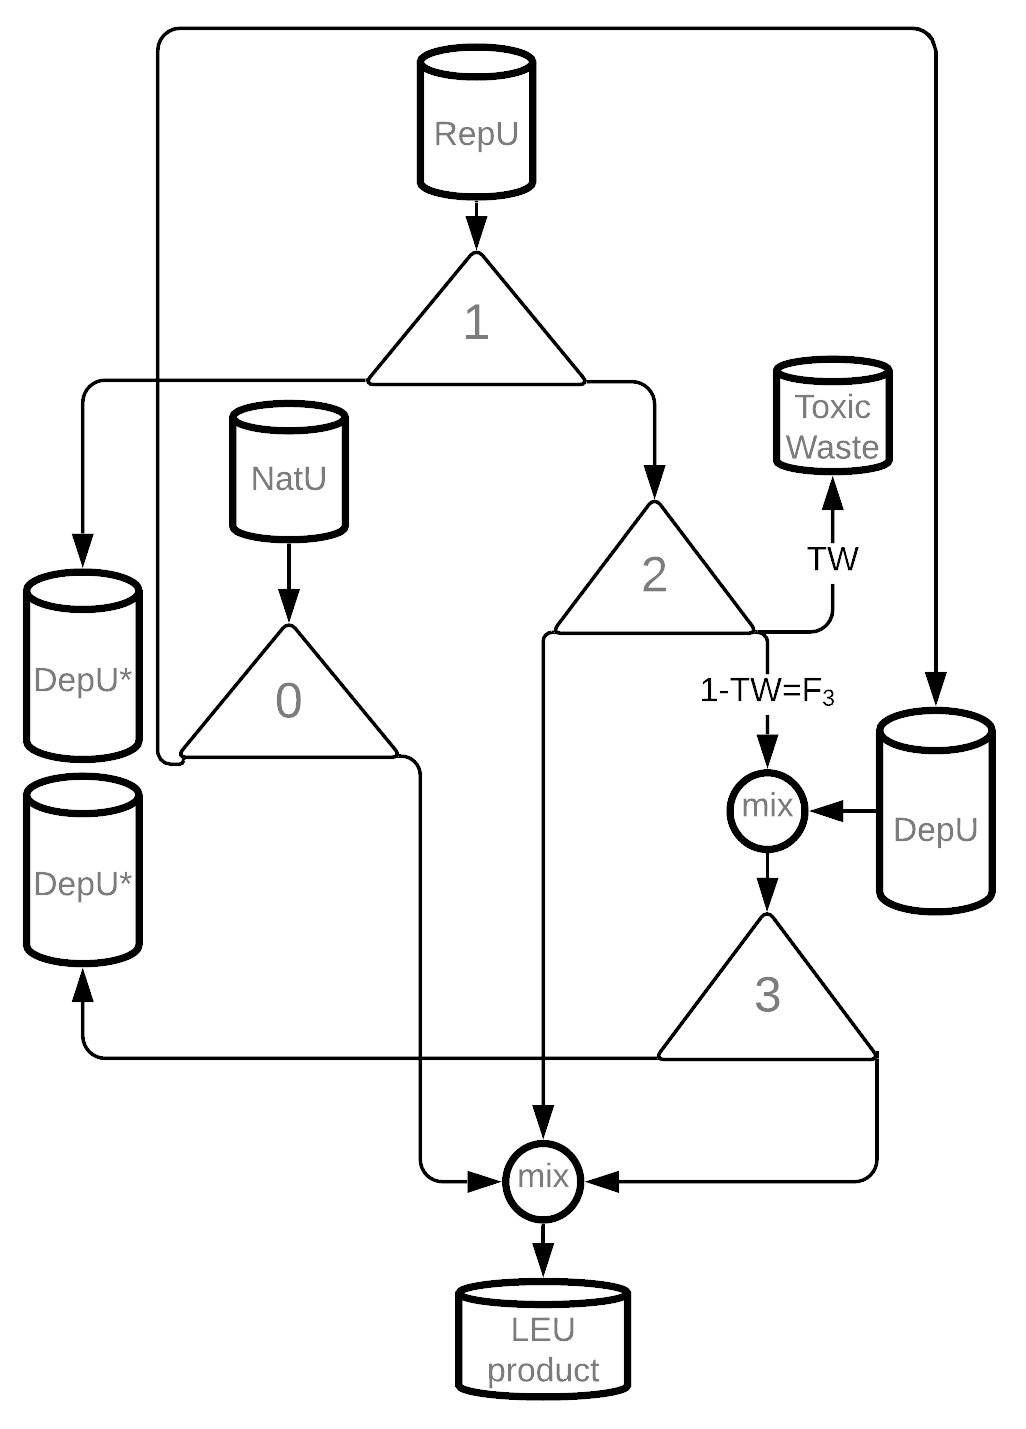
\includegraphics[scale=0.3]{cascades/Triple_Tomsk}}
  \caption{Тройной каскад с подмешиванием ОГФУ и НОУ-разбавителем}\label{fig:Tomsk}
\end{figure}

Затем, в качестве альтернативы была предложена схема рисунка \ref{fig:patent}), в которой на каскад с индексом 3 подается смесь грязного потока легкой фракции каскада 2, которая разбавляется обедненным гексафторидом урана до содержания $^{235}$U на уровне природного урана. Этот поток в дальнейшем разбавляется чистым природным ураном, пропорция которого подбирается для выполнения всех заданных условий.
\begin{figure}[ht]
  \centerfloat{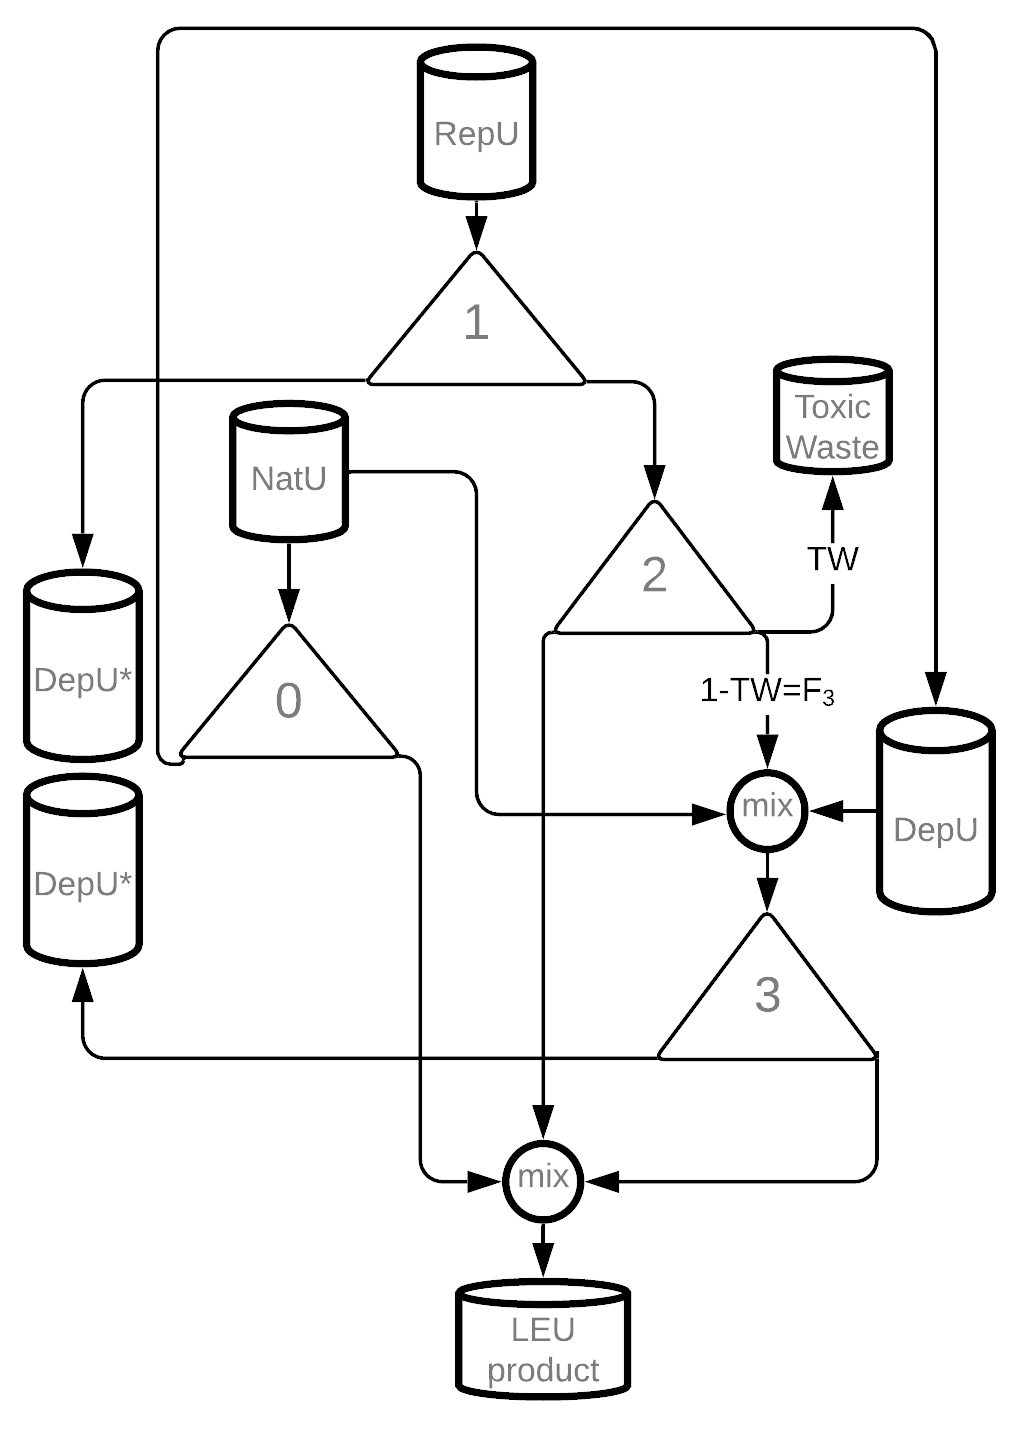
\includegraphics[scale=0.3]{cascades/triple_cascade_complete_return}}
  \caption{Тройной каскад с подмешиванием НОУ, ОГФУ и природного урана}\label{fig:patent}
\end{figure}

Как мы видим, такие схемы также очень ценны как инструмент для переработки предписанного количества выделенного урана.

Хранение загрязненного побочного продукта сопряжено с существенными дополнительными затратами, поэтому важен поиск способов избежать накопления этого материала.
Исходя из этого, в работе \cite{smirnovMethodEnrichReprocessed2019} предложено применить дополнительный каскад.
Далее будет предложен краткий обзор такого каскада.

\subsection{Четверной каскад}

Схема каскада, состоящего из четырех ординарных каскадов решает проблему обращения с легкой фракцией, вышедшей из второго каскада.
Это позволяет вовлечь больше $^{235}$U, и избавляет от необходимости конечной утилизации материала с высоким содержанием $^{232}$U.
Принцип работы такой схемы состоит в следующем.
Теперь финальный продукт -- низкообогащенный уран -- получается путем смешения двух потоков.
Первый из них аналогичен финальному продукту, полученному посредством тройной схемы рис. \ref{fig:triple}.
Второй же нарабатывается из загрязненной смеси, сильно разбавленной обедненным ураном.
При этом, конфигурация подбирается таким образом, чтобы на получение единицы продукта из этих совмещенных потоков затрачивалось требуемое количество ($\approx$0.93) питающего регенерата.

Итак, данная схема позволяет получить конечный продукт в двух исходящих потоках и достичь значительной экономии природного урана (~ 38\%) даже для «грязного» регенерата, которая уже была пятикратно переработана.
При этом, для того же исходного состава регенерата, тройная схема показывает лишь (~ 8\%) в сокращении расхода природного урана в сравнении с ординарным, обогащающим природный уран \cite{smirnovObogashchenieRegenerirovannogoUrana2018}.
Однако такой эффект связан с двухкратной работой разделения, требуемой четверной схеме, тогда как тройная схема затрачивает лишь (~ 13\%) дополнительных РР.
Это связано с большим объемом вовлечения ОГФУ для разбавления загрязненного потока легкой фракции второго каскада.
Расчеты показали, что такой подход позволяет производить НОУ коммерческого качества, расходуя должное количество переработанного урана, в то же время отвечая стандартным спецификациям $^{232}$U (и условиям, установленным для других четных изотопов).
В то же время, предлагаемая схема обеспечивает более существенную экономию природного урана, чем большинство схем обогащения регенерированного урана.
Такая схема позволяет также обеспечить широкомасштабную «мобилизацию» обедненного урана.

\section{Сравнение схем полного возврата}

В данной части проводится сравнительный анализ каскадов, предназначенных для возврата регенерированного урана в ЯТЦ.
Рассматривается случай, когда схема производит эквивалентное количество продукта НОУ, затраченному регенерату.
Чтобы моделировать многократную переработку ядерного топлива, в качестве сырья используется регенерат, прошедший пять последовательных циклов.
Ключевые характеристики, связанные с общей эффективностью, такие как экономия природного урана, расход работы разделения и энергозатраты, были оценены для каждой схемы в удельных единицах (на единицу продукции).
Затем они были нормированы на величины, характерные для ординарного каскада(трехпоточного).
Чтобы избежать стоимостных показателей затрат, была использована методология пересчета ключевых показателей (экономия природного урана, объем обогащаемого ОГФУ и затраты работы разделения) в единицы потребляемой энергии (мегаватт-часы)  \cite{rodionovaAnalizTehnikoekonomicheskihHarakteristik2019}.
Этот показатель был предложен в качестве универсального инструмента оценки рассматриваемых каскадов, используемых для повторного обогащения урана.


